% ------------------------------
% Aufgabenteil 3 - Aussage 1
% ------------------------------
\begin{figure}[H]
	\centering
		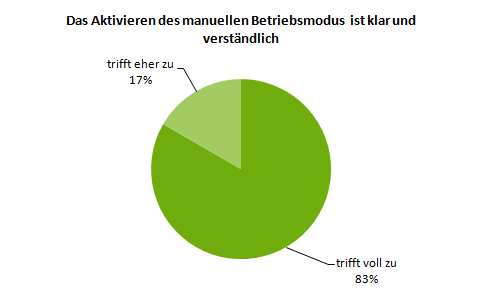
\includegraphics[width=0.85\textwidth]{03_Grafiken/Anhang/UsabilityDiagramme/Aufgabenteil3Aussage1.png}
	\caption[Diagramm zum Analysieren der Benutzerfreundlichkeit beim Verfahren mit Pfeiltasten - Aussage 1]{Diagramm zum Analysieren der Benutzerfreundlichkeit beim Verfahren mit Pfeiltasten - Aussage 1}
	\label{fig:Aufgabenteil3Aussage1}
\end{figure}
% ------------------------------
% Aufgabenteil 3 - Aussage 2
% ------------------------------
\begin{figure}[H]
	\centering
		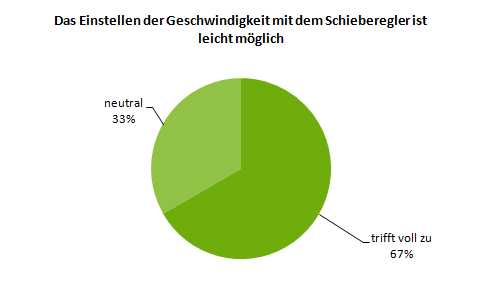
\includegraphics[width=0.85\textwidth]{03_Grafiken/Anhang/UsabilityDiagramme/Aufgabenteil3Aussage2.png}
	\caption[Diagramm zum Analysieren der Benutzerfreundlichkeit beim Verfahren mit Pfeiltasten - Aussage 2]{Diagramm zum Analysieren der Benutzerfreundlichkeit beim Verfahren mit Pfeiltasten - Aussage 2}
	\label{fig:Aufgabenteil3Aussage2}
\end{figure}
% ------------------------------
% Aufgabenteil 3 - Aussage 3
% ------------------------------
\begin{figure}[H]
	\centering
		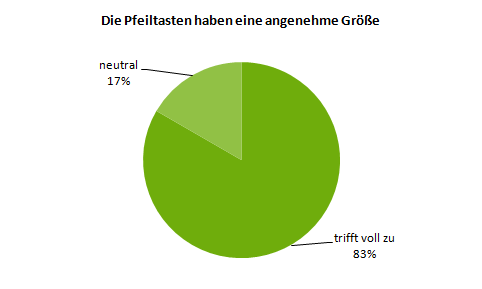
\includegraphics[width=0.85\textwidth]{03_Grafiken/Anhang/UsabilityDiagramme/Aufgabenteil3Aussage3.png}
	\caption[Diagramm zum Analysieren der Benutzerfreundlichkeit beim Verfahren mit Pfeiltasten - Aussage 3]{Diagramm zum Analysieren der Benutzerfreundlichkeit beim Verfahren mit Pfeiltasten - Aussage 3}
	\label{fig:Aufgabenteil3Aussage3}
\end{figure}
% ------------------------------
% Aufgabenteil 3 - Aussage 4
% ------------------------------
\begin{figure}[H]
	\centering
		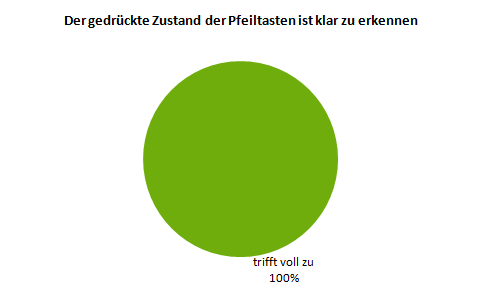
\includegraphics[width=0.85\textwidth]{03_Grafiken/Anhang/UsabilityDiagramme/Aufgabenteil3Aussage4.png}
	\caption[Diagramm zum Analysieren der Benutzerfreundlichkeit beim Verfahren mit Pfeiltasten - Aussage 4]{Diagramm zum Analysieren der Benutzerfreundlichkeit beim Verfahren mit Pfeiltasten - Aussage 4}
	\label{fig:Aufgabenteil3Aussage4}
\end{figure}
% ------------------------------
% Aufgabenteil 3 - Aussage 5
% ------------------------------
\begin{figure}[H]
	\centering
		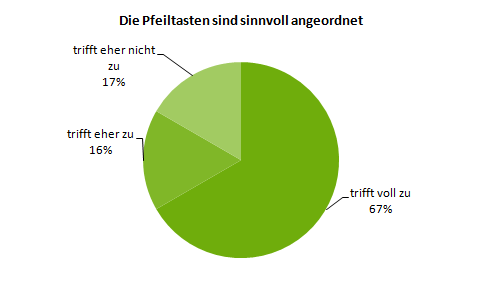
\includegraphics[width=0.85\textwidth]{03_Grafiken/Anhang/UsabilityDiagramme/Aufgabenteil3Aussage5.png}
	\caption[Diagramm zum Analysieren der Benutzerfreundlichkeit beim Verfahren mit Pfeiltasten - Aussage 5]{Diagramm zum Analysieren der Benutzerfreundlichkeit beim Verfahren mit Pfeiltasten - Aussage 5}
	\label{fig:Aufgabenteil3Aussage5}
\end{figure}
% ------------------------------
% Aufgabenteil 4 - Aussage 1
% ------------------------------
\begin{figure}[H]
	\centering
		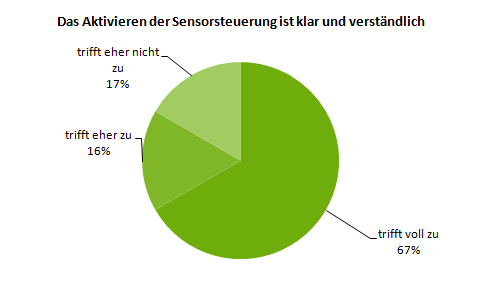
\includegraphics[width=0.85\textwidth]{03_Grafiken/Anhang/UsabilityDiagramme/Aufgabenteil4Aussage1.png}
	\caption[Diagramm zum Analysieren der Benutzerfreundlichkeit bei der Sensorsteuerung - Aussage 1]{Diagramm zum Analysieren der Benutzerfreundlichkeit bei der Sensorsteuerung - Aussage 1}
	\label{fig:Aufgabenteil4Aussage1}
\end{figure}
% ------------------------------
% Aufgabenteil 4 - Aussage 2
% ------------------------------
\begin{figure}[H]
	\centering
		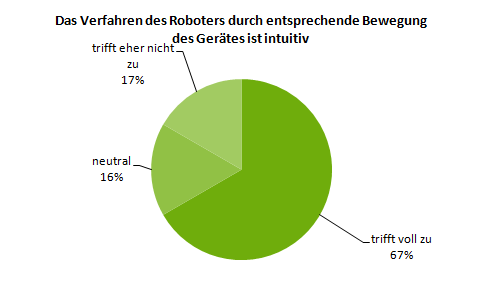
\includegraphics[width=0.85\textwidth]{03_Grafiken/Anhang/UsabilityDiagramme/Aufgabenteil4Aussage2.png}
	\caption[Diagramm zum Analysieren der Benutzerfreundlichkeit bei der Sensorsteuerung - Aussage 1]{Diagramm zum Analysieren der Benutzerfreundlichkeit bei der Sensorsteuerung - Aussage 2}
	\label{fig:Aufgabenteil4Aussage2}
\end{figure}
% ------------------------------
% Aufgabenteil 4 - Aussage 2
% ------------------------------
\begin{figure}[H]
	\centering
		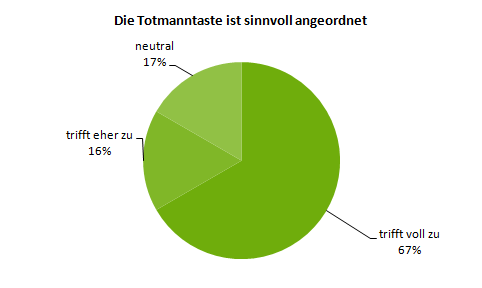
\includegraphics[width=0.85\textwidth]{03_Grafiken/Anhang/UsabilityDiagramme/Aufgabenteil4Aussage4.png}
	\caption[Diagramm zum Analysieren der Benutzerfreundlichkeit bei der Sensorsteuerung - Aussage 4]{Diagramm zum Analysieren der Benutzerfreundlichkeit bei der Sensorsteuerung - Aussage 4}
	\label{fig:Aufgabenteil4Aussage4}
\end{figure}
% ------------------------------
% Aufgabenteil 5 - Aussage 2
% ------------------------------
\begin{figure}[H]
	\centering
		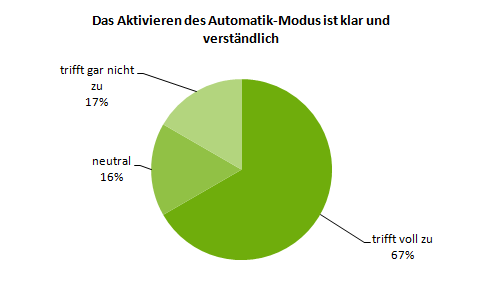
\includegraphics[width=0.85\textwidth]{03_Grafiken/Anhang/UsabilityDiagramme/Aufgabenteil5Aussage1.png}
	\caption[Diagramm zum Analysieren der Benutzerfreundlichkeit im Automatik-Modus - Aussage 1]{Diagramm zum Analysieren der Benutzerfreundlichkeit im Automatik-Modus - Aussage 1}
	\label{fig:Aufgabenteil5Aussage1}
\end{figure}
% ------------------------------
% Aufgabenteil 5 - Aussage 2
% ------------------------------
\begin{figure}[H]
	\centering
		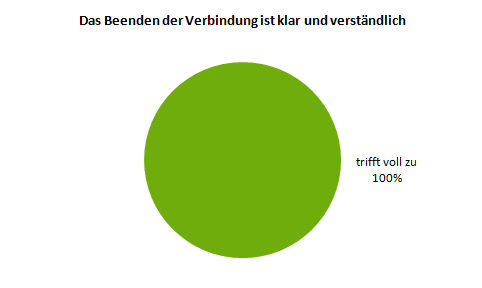
\includegraphics[width=0.85\textwidth]{03_Grafiken/Anhang/UsabilityDiagramme/Aufgabenteil5Aussage2.png}
	\caption[Diagramm zum Analysieren der Benutzerfreundlichkeit im Automatik-Modus - Aussage 2]{Diagramm zum Analysieren der Benutzerfreundlichkeit im Automatik-Modus - Aussage 2}
	\label{fig:Aufgabenteil5Aussage2}
\end{figure}